\setchapterpreamble[u]{\margintoc}
\chapter{History: The End of Good Old-Fashioned Artificial Intelligence}
\labch{intro}

\textit{"Programming will be obsolete. I believe the conventional idea of "writing a program" is headed for extinction, and indeed, for all but very specialized applications, most software, as we know it, will be replaced by AI systems that are trained rather than programmed. In situations where one needs a "simple" program (after all, not everything should require a model of hundreds of billions of parameters running on a cluster of GPUs), those programs will, themselves, be generated by an AI rather than coded by hand."} Matt Welsh, 2023 \cite{welsh2023}

\section{The AI Textbook in 1997}

Dr. Elaine Rich's textbook on artificial intelligence (AI), published in the 1980s, was a groundbreaking work that helped to establish many of the core concepts and techniques in the field of AI. However, the rapid advancements in AI over the past few decades have led to many of the chapters in this textbook becoming obsolete.

One of the main reasons for this is the prevalence of deep learning, big data, and large-scale statistical models in modern AI. These techniques have largely replaced the symbolic, rule-based approach to AI that was emphasized in the textbook, making many of the chapters on knowledge representation and expert systems less relevant.

Additionally, the explosion of data and the availability of powerful computing resources have made it possible to apply machine learning techniques at a scale that was previously unimaginable. This has led to the development of highly effective machine learning models that can handle complex tasks such as image and speech recognition with a high degree of accuracy, making many of the chapters on simpler machine learning techniques such as decision trees\sidenote{Although mathematically neural networks are decision trees \url{https://arxiv.org/abs/2210.05189}} and linear regression less relevant. \sidecite{rich_2009} \sidenote{the book is now in its third edition and unlikely to be updated as Dr. Rich as retired \url{https://www.cs.utexas.edu/~ear/}}


We'll discuss this history and a few examples from the "early days" of AI to help us understand where we are headed. We'll start with machine translation, then discuss chess and finally neural networks, which will be the focus of the rest of this book.

\section{Does AI Need to Know Grammar to Translate?}

Noam Chomsky is a linguist and philosopher who has made significant contributions to the field of linguistics with his theory of universal grammar. Chomsky believes that all human languages share a common underlying structure, and that this structure is innate to humans. He proposes that this innate structure is the result of a "language acquisition device" present in the human brain, which allows us to learn and produce language. Chomsky also argues that the structure of language is largely independent of its content, and that the ability to produce and understand language is a fundamental aspect of human nature. His theory has been influential in the field of linguistics and has sparked much debate and research on the nature of language and its relationship to the human mind.

For English speakers or anyone who has learned English as a second language you'll have many examples of special cases, irregular verbs, bad English and former street slang that became good and proper over time. For programmers this is a nightmare, how can we codify human knowledge in a timely fashion? If we tried to write the rules of the English language in code (which many have tried to do) the rules themselves might change before we were finished writing them.

Explicitly translating languages through code is a difficult task because it requires a thorough understanding of the grammar, vocabulary, and syntax of both languages, as well as the nuances and subtleties of their respective cultures\sidenote{For programmers this is a nightmare, how can we codify human knowledge in a timely fashion? If we tried to write the rules of the English language in code (which many have tried to do) the rules themselves might change before we were finished writing them.}. Simply coding rules for how to translate words or phrases from one language to another is not sufficient, as there are often multiple valid translations for a given phrase depending on the context in which it is used.

A more effective approach to translation is to use statistical techniques that rely on a large corpus of translated data, such as Canadian laws\sidenote{They're in French AND English, which is useful data that we can use to correlate phrases and transform English to French and vice-versa.}. This type of data-driven approach involves training a machine learning model on a large dataset of translations, allowing it to learn the patterns and relationships between the languages. The model can then use this knowledge to make educated translations of new phrases or sentences, taking into account the context in which they are used.

While this approach is not perfect, it has proven to be highly effective in machine translation and can produce accurate translations even for languages that are very different from each other. The use of a large dataset of translations also allows the model to learn from the mistakes and variations present in real-world translations, further improving its accuracy.

\section{Explicit Rules and Codified Human Knowledge}

When we "teach" a computer to perform a task by explicitly writing down all of the rules of that task, we are really codifying human understanding.\sidenote{Programming this way makes some software development totally boring, I almost switched my major in college to math after considering what a life would look like manually writing rules for handling "edge cases" for the rest of my natural life.} When we codify human understanding we write down every rule that we know explicitly. For small tasks we can do this with 100 percent accuracy, and only minor headache on the part of the software developer. 

For example, let's write a boring function to tell you the number of days for a given month. 

\begin{lstlisting}[language=Python,style=kaolstplain,linewidth=1.5\textwidth]
def days_in_month(year, month):
  if month in [1, 3, 5, 7, 8, 10, 12]:
    return 31
  elif month in [4, 6, 9, 11]:
    return 30
  elif month == 2:
    if (year % 4 == 0 and year % 100 != 0) or year % 400 == 0:
      return 29
    else:
      return 28
  else:
    return "Invalid month"

\end{lstlisting}


Writing code can be a tedious and repetitive task, especially when it comes to debugging and testing. It can be especially frustrating when you're working on a large project and you're trying to track down a specific bug that's causing the program to crash. Testing code can also be boring, as it often involves running the same tests over and over again to ensure that the code is working correctly.

Additionally, writing code can be boring because it requires a lot of concentration and focus. It can be easy to get lost in the details and lose track of time, especially if you're working on a complex problem. It can also be challenging to come up with creative solutions to problems, and it can be frustrating when your code doesn't work as expected.

\begin{marginfigure}[-5.5cm]
        
\includegraphics{bored_programmer}
        \caption{"a frustrated programmer writing boring rules on his computer" made with Stable Diffusion 2.1}
        \labfig{marginprogrammer}
\end{marginfigure}

While writing and testing code can be rewarding and fulfilling, it can also be a tedious and boring process. It requires a lot of patience, persistence, and attention to detail, and it can be easy to get frustrated and lose motivation. However, with practice and perseverance, it is possible to overcome these challenges and find enjoyment in the process of writing and testing code.

AI has traditionally operated by explicitly codifying human knowledge into machine-readable formats by doing the boring job of coding. This approach, which I'm calling "codified human knowledge" relies on humans to carefully structure and organize information in a way that can be understood by the AI system. The AI system then uses this structured knowledge to make decisions and perform tasks.\sidenote{Some smart people think that AI spells the "End of Programming" \url{https://cacm.acm.org/magazines/2023/1/267976-the-end-of-programming/fulltext}, I think the headline is clickbait but the general idea that programming is changing along with advances in AI is true. We are all data scientists now!}

However, recent advances in AI have largely ignored the knowledge representation problem and instead have focused on using statistical techniques and neural networks to automatically learn patterns and relationships in data. This approach, known as "deep learning," involves training large neural networks on vast amounts of data, allowing the AI system to make educated classifications and transformations of data without explicit human guidance.

Deep learning has proven to be highly effective in a variety of applications, such as image and speech recognition, and has contributed to the rapid progress we have seen in AI in recent years. However, the reliance on large amounts of data and the lack of transparency in these models can make it difficult to understand how they are making decisions, which can be a concern in certain applications (hence the title of this book).

\section{IBM Tries Every Possible Chess Move}

Deep Blue was a revolutionary computer developed by IBM that was specifically designed to play chess at the highest level. It was programmed with a vast database of chess knowledge and was able to analyze millions of positions per second.

Garry Kasparov was the reigning world chess champion at the time, and he was considered to be one of the greatest players in history. He was beaten by Deep Blue, which used rules based GOFAI (Good Old Fashioned AI) to essentially calculate every possible move and project that move to the end of the game, then choose the best position by brute force. Despite Kasparov's best efforts, he was no match for Deep Blue's computational power. In the end, Deep Blue emerged victorious, defeating Kasparov in a historic match that changed the world of chess forever.

\begin{marginfigure}[-5.5cm]
        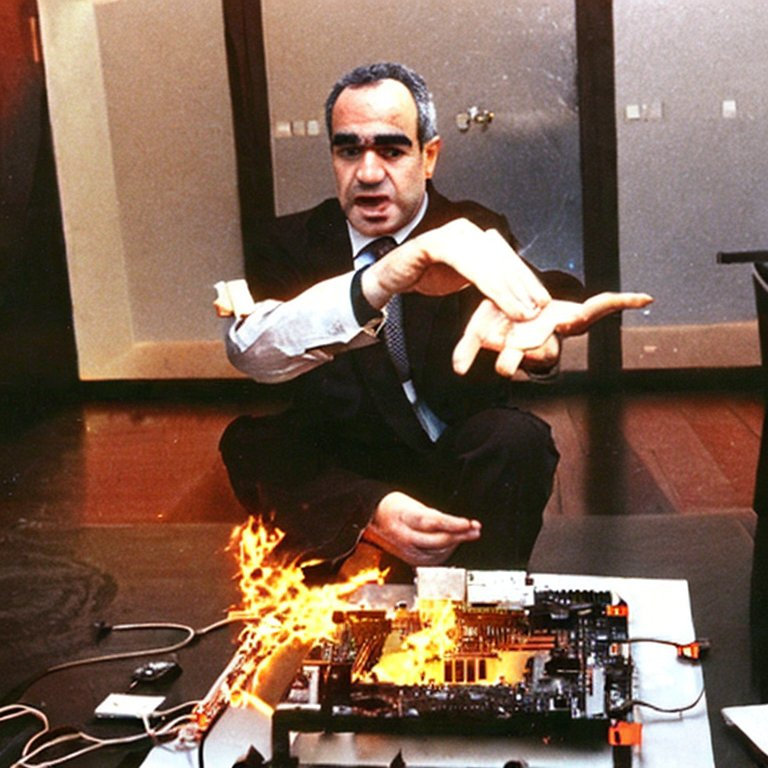
\includegraphics{kasparov_fire}
	\caption{"Garry Kasparov setting a computer on fire" made with Stable Diffusion 2.1}
        \labfig{marginkasparov}
\end{marginfigure}

Deep Blue was a turning point in the development of AI, but Deep Blue's methods (namely calculating every possible outcome of a Chess game to determine the best move) was not suitable for many of the world's problems. It turns out that Chess is fun, but the world is not like chess.\sidenote{if you would like to read an example of the simplest chess engine that I could imagine that is written in a similar "codified" way as Deep Blue check out \url{https://github.com/thomasahle/sunfish/blob/master/sunfish.py}} The "real"\sidenote{We might go back, and try again to more explicitly code everything up, and in some cases we still need to, but from the author's perspective, we live in a deep learning/neural network world.} future of AI was being developed elsewhere, using statistics and a toy model of the brain to solve a very practical problem for banks.

\section{Statistical Analysis of Handwriting is the Way of the Future}

It was the early 1990s and Yann LeCun was a researcher at Bell Labs in New Jersey. At the time, the process of reading and processing checks was a tedious and time-consuming task that was done manually by bank employees. LeCun saw the potential for using artificial intelligence to automate this process, and he began experimenting with using convolutional neural networks (CNNs) to recognize patterns in images of checks.

At the time, CNNs were a relatively new type of neural network that had been developed in the 1980s for image recognition tasks. They were inspired by the structure of the human visual system, and were able to process images in a way that was similar to how the human brain does.

LeCun's work was groundbreaking, and he was able to achieve impressive results using CNNs to process checks. By 1993, he had developed a system that was able to read and process checks with a high degree of accuracy, significantly reducing the amount of time and effort that was required to process checks manually.\sidenote{CNN digit OCR models are frequently featured in beginner training tutorials for deep learning libraries like PyTorch and Tensorflow, check one out \url{https://github.com/jonkrohn/DLTFpT/blob/master/notebooks/alexnet_in_tensorflow.ipynb}}

LeCun's work on using CNNs for check processing was a major milestone in the field of artificial intelligence, and it laid the foundation for the development of many other applications of CNNs in the years that followed. Today, CNNs are widely used in a variety of applications, including facial recognition, image classification, and natural language processing. \sidenote{check out Yann LeCun domonstrating a convolutional neural network in 1993 at \url{https://www.youtube.com/watch?v=FwFduRA_L6Q}.}

\section{Less Programmer Intelligence and More Data Intelligence}

I think it's useful to separate the knowledge in the AI problem-space into two groups. The data and the programmer together make the programs that we use every day, and for the rest of this book I'll try and separate the discussion of the smarts of each to help us better understand the world. \sidenote{I'll also repeatedly encourage you to use the words "algorithm" and "artificial intelligence" sparingly. They'll confuse your thinking, I promise.}

Early AI relied heavily on a human programmer to design, write, and debug computer programs. Good programmers needed domain expertise, problem-solving skills, logical thinking, and the ability to learn and adapt to new programming languages and technologies.

We are now in the age of big data, and everyone knows that "data is gold". Statistical AI methods that are now most prevalent rely on extracting meaningful insights and knowledge from large datasets. This involves using statistical and analytical methods to discover patterns and trends in data, and using this information to inform business decisions or solve problems. 

\begin{marginfigure}[-5.5cm]
        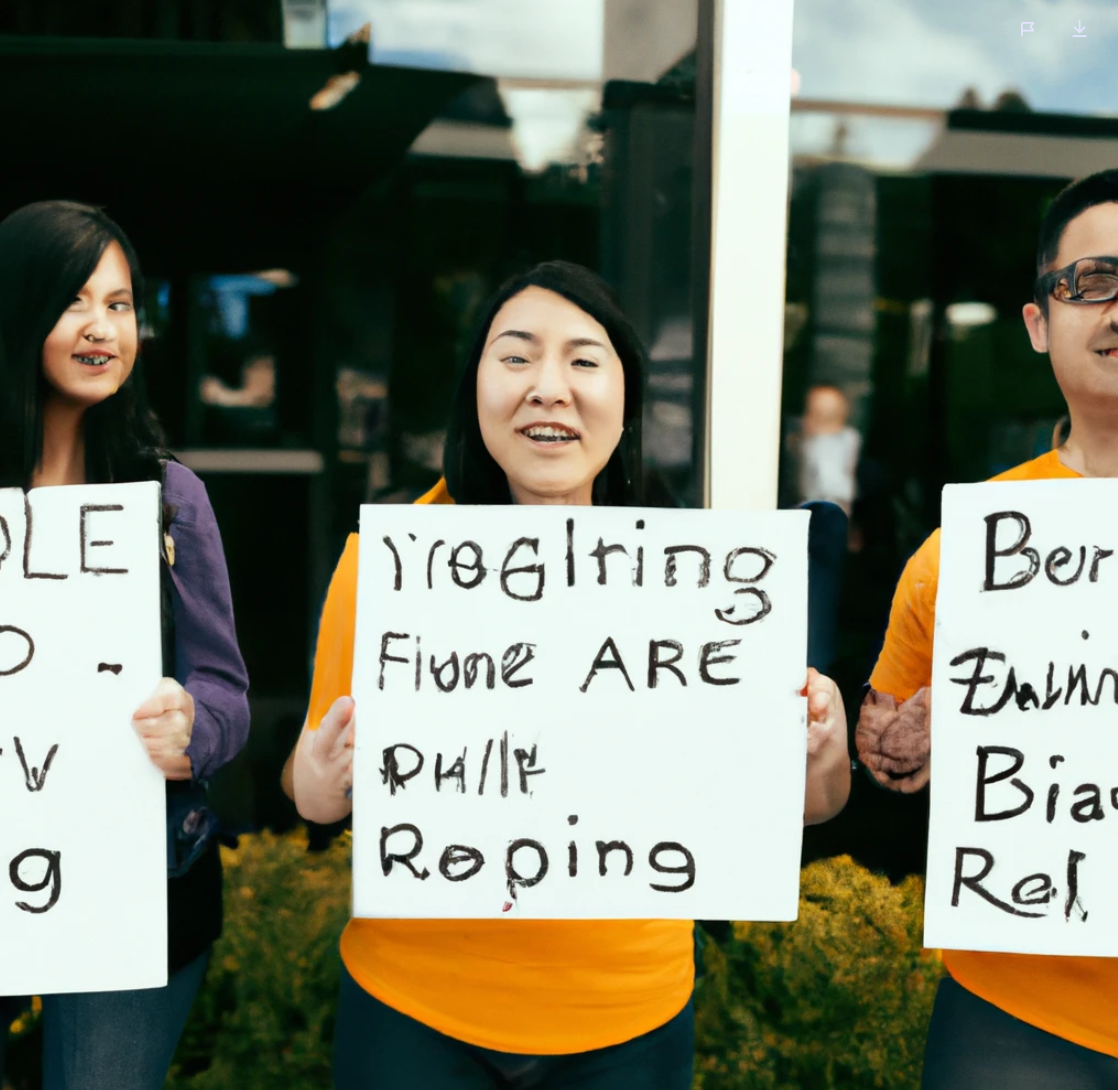
\includegraphics{programmers_strike}
        \caption{"a group of computer programmers striking outside of Microsoft's offices with placards saying 'rule-based programming is boring'" made with Dall-E 2}
        \labfig{marginprogrammersstrike}
\end{marginfigure}

Throughout this book I'll discuss the interaction between programmer and data, and what can go wrong. Working with big data and statistics at a large scale has given AI tremendous ability, but has made understanding and testing models infinitely more difficult. It is your authors belief that understanding the nuance of this interaction between programmer and data is essential to understanding modern AI.

\section{From Explicit Rules to a Black Box, and Beyond}

Artificial intelligence (AI) has come a long way since its inception, and the way that it makes decisions has changed significantly over time. In the early days of AI, explicit rules were used to tell the AI system what to do in certain situations. These rules were often written by humans and encoded into the system, and the AI would follow them to make decisions.

However, with the advent of deep learning, we have started to rely on a statistical understanding of the truth for AI to make decisions. Deep learning is a type of machine learning that involves training artificial neural networks on large datasets. These neural networks are able to learn patterns and relationships in the data, and can use this knowledge to make decisions.

The use of deep learning has led to the development of powerful AI that is able to perform tasks that were previously thought to be impossible for a machine to handle. For example, deep learning has led to the development of AI systems that are able to recognize faces, translate languages, and even beat humans at complex games like chess and Go.

\begin{marginfigure}[-5.5cm]
        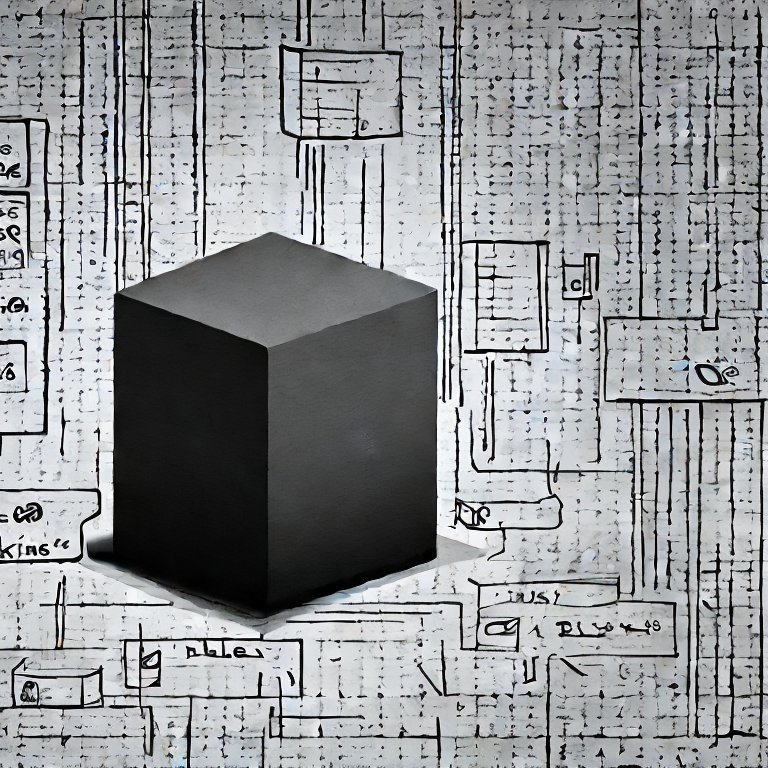
\includegraphics{blackbox}
        \caption{"from explicit rules, to a black box and beyond" made with Stable Diffusion 2.1}
        \labfig{marginblackbox}
\end{marginfigure}

While deep learning has led to significant advances in AI, it has also made it harder to debug and understand how the AI system is making its decisions. With explicit rules, it was relatively easy to understand why the AI made a particular decision. However, with deep learning, it is often difficult to understand exactly how the AI arrived at its decision. This can make it challenging to troubleshoot problems with the AI system and to ensure that it is making decisions that are fair and unbiased.

AI has come a long way since its early days, and the way that it makes decisions has changed significantly over time. While explicit rules were once used to tell the AI what to do, we now rely on a statistical understanding of the truth for AI to make decisions. This has led to the development of powerful AI that is able to perform a wide range of tasks, but it has also made it harder to debug and understand how the AI is making its decisions.\sidenote{From here on out I'll try and use "GOFAI" (Good Old-Fashioned Artificial Intelligence) to describe the rules-based approach, and use "Deep Learning" or "Machine Learning" to talk about modern neural network and statistics-based techniques}

\section{Key Takeaways}

\begin{itemize}
	\item \textbf{AI is a misleading term}, we should instead talk about rules-based programming (GOFAI) and deep learning so we don't confuse ourselves, our partners and our users.\sidenote{Avoid the imprecise words "Algorithms" and "AI" and instead consider the more precise "rules-based AI" AKA "GOFAI" to describe situations where programmers explicitly write rules that they design and "deep learning" or "machine learning" where programmers create models using a dataset and let the machine figure out the rules via a neural network.} 
	\item Good Old-Fashioned AI \textbf{(rules-based AI) is hard to create and maintain}. We used to use it for chess engines (like Deep Blue) and translation, but now programmers favor using statistical machine learning techniques.
	\item Good Old-Fashioned AI is not well suited to many problems, like machine translation and handwriting detection.
	\item Modern Deep Learning techniques use data to train models instead of humans explicitly writing rules, and the \textbf{deep learning models are often as good as the data they are trained with}.\sidenote{More \textit{intelligent} data and maybe less intelligent programmers, or maybe programmers who are better trained in statistics and complex systems theory instead of "classical" computer science.}
\end{itemize}
